
\addcontentsline{toc}{subsection}{Cleaning the Data}
\subsection*{Cleaning the Data}

Attempts at cleaning the data were made by neglecting terms outside of the
center regions on the Y-axis of 2D histogram plots of rapidity, transverse momentum of the muon pair, and the transverse momentum of each of
the individual muons against the invariant mass. The results of which were tested using the ratios method discussed in the methods section, showing that none of these showed any sign of cleaning the data, as both ratios were equal. This was to be expected, as none of the measured properties alone have any direct correlation to the origin of the signal. \\

The previously described cleaning method using the R-value was also implemented. First, the a graph showing the the correlation between the two muon pair momenta was plotted.

\begin{figure}[H]
\centering
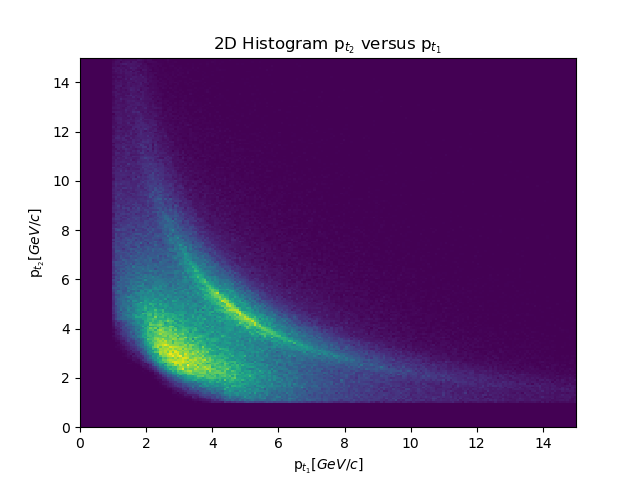
\includegraphics[width=0.7\columnwidth]{figures/mom_tran_1_2_2d_hist.png}
\caption{Graph of the transverse momenta of the two particles plotted against each other. Counts close to the 45$^o$ line are the counts of interest.}
\label{fig:2d_hists_ex}
\end{figure}

Values for R were calculated and plotted against the invariant muon pair mass.

\begin{figure}[H]
\centering
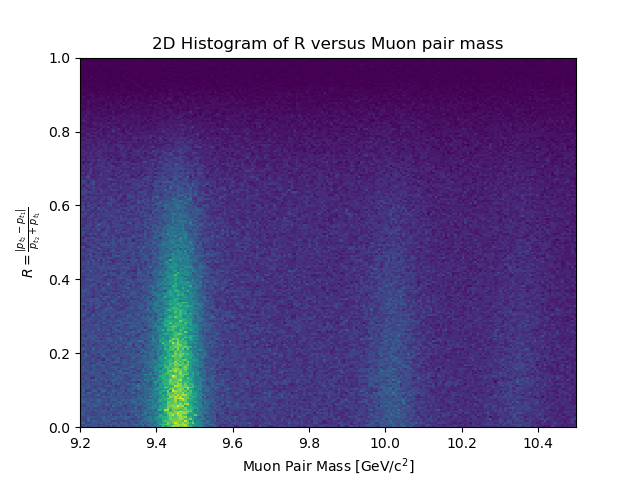
\includegraphics[width=0.7\columnwidth]{figures/xmass_sub_mom_tran_1_2_2d_hist.png}
\caption{R values against muon pair mass, showing the concentration of values at the peak region with low values of R, and relatively homogeneous counts in the background region.}
\label{fig:2d_hists_ex}
\end{figure}

From this, we made an initial estimation that a cutoff value of R=0.5 would be sufficient, however to be more rigorous, we decided to look at the spread of R values across the background regions and across the first peak region. The first peak region was used as this is the only peak that has sidebands that are unaffected by other peaks. 

\begin{figure}[H]
\centering
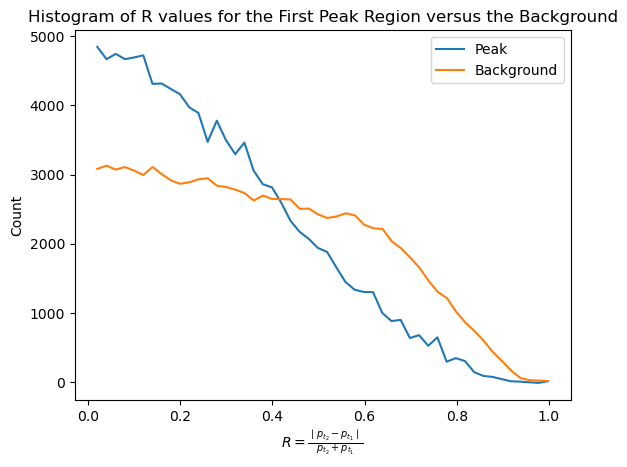
\includegraphics[width=0.6\columnwidth]{figures/r_val_graph.png}
\caption{Spread of R values across the first peak region and a background region, showing an obvious difference in shape of the curves.}
\label{fig:2d_hists_ex}
\end{figure}

This figure confirmed that the theory of the R value was successful in differentiating between signals from decays and background signals. Furthermore, the crossover point of roughly R=0.42 was taken to be a good cutoff value. So any signal with R$>$0.42 was discarded.\\

\begin{figure}[H]
\centering
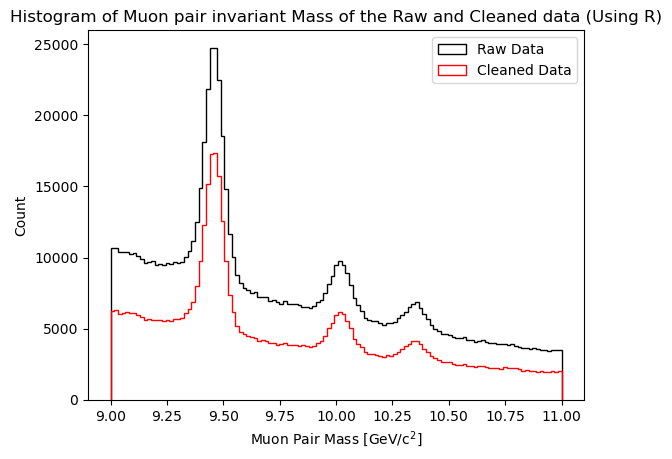
\includegraphics[width=0.6\columnwidth]{figures/cleaned_hist.png}
\caption{Histograms of the original data and the cleaned data}
\label{fig:2d_hists_ex}
\end{figure}

The resulting data was analysed by using the same ratios method. The results of which showed the background decreased by a factor of 1.705 whereas the peak region decreased by a factor of only 1.523, showing the data had been obviously cleaned. This cleaned data was then binned in a histogram and was used for the analysis in the report from this point onward.

\addcontentsline{toc}{subsection}{Exponential Background Fit}
% in the new method I m not actually taking the 
\subsection*{Exponential Background Fit}

The background regions were isolated and fitted with an exponential decay PDF (see equation (5)). The parameters of the PDF were
optimised using a negative log likelihood within PyRoot’s Fit() method.


\begin{figure}[H]
\centering
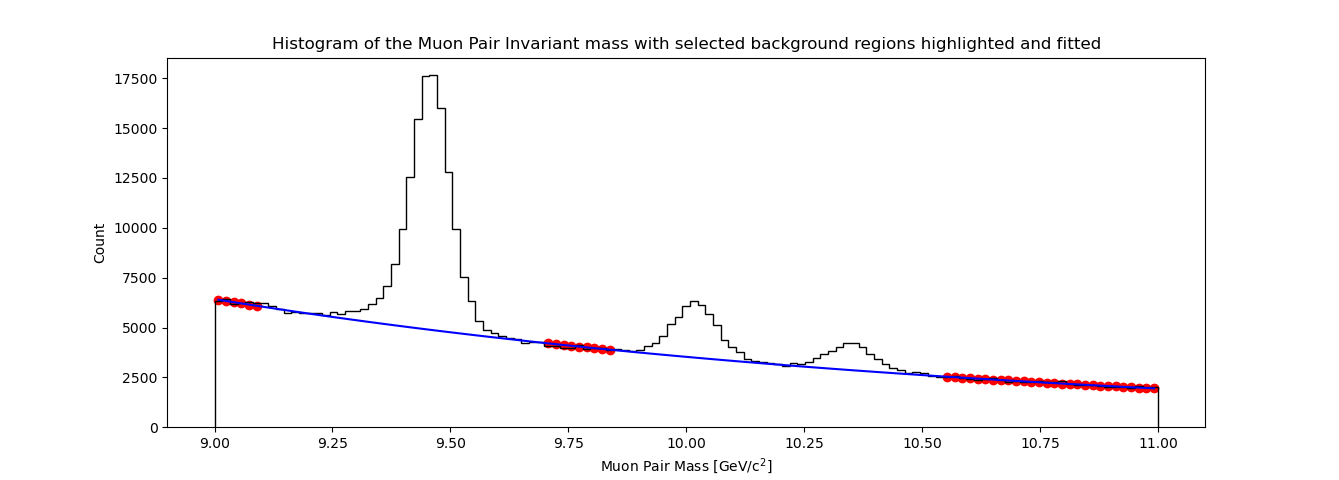
\includegraphics[width=0.9\columnwidth]{figures/expo_high_hist.png}
\caption{Histogram showing, in red, the points from which the exponential decay function was calculated. The fitted curve is also shown in blue.}
\label{fig:2d_hists_ex}
\end{figure}



\addcontentsline{toc}{subsection}{Gaussian Fit}
\subsection*{Gaussian Fit}

The PDF constructed to fit the data with Gaussian curves was the sum of three Gaussian's (equation 6) and an exponential decay (equation 5). All parameters of the PDF were optimised simultaneously using a negative log likelihood within PyRoot's \verb|Fit()| method.

\begin{figure}[H]
\centering
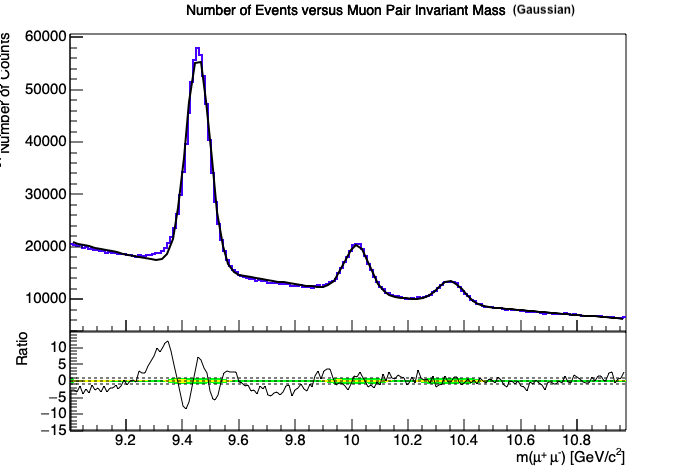
\includegraphics[width=0.7\columnwidth]{figures/xmass_hist_gauss.png}
\caption{Histogram showing the Gaussian curves fit to the three peaks, along with the exponential background fit.}
\label{fig:2d_hists_ex}
\end{figure}

Something to note about this graph is the excess of measurements on the low end of the first peak. The other models will attempt to rectify this discrepancy between the fit and the data. The reduced $\chi ^2$ was determined to be 9.976 for the single Gaussian fit.



\addcontentsline{toc}{subsection}{Double Gaussian Fit}
\subsection*{Double Gaussian Fit}

The PDF constructed to fit the peaks to Double Gaussian curves was the sum of three Double Gaussian's (equation 7) and an exponential decay (equation 5). All parameters of the PDF were optimised simultaneously using a negative log likelihood within PyRoot's \verb|Fit()| method. 

\begin{figure}[H]
\centering
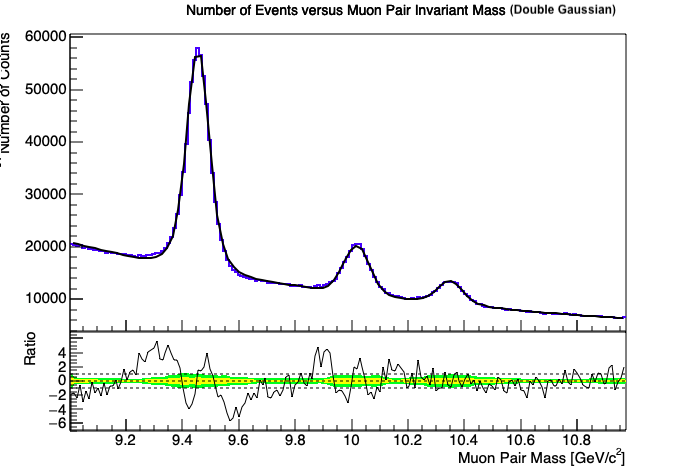
\includegraphics[width=0.7\columnwidth]{figures/xmass_hist_d_gauss.png}
\caption{Histogram showing the double Gaussian curves fit to the three peaks, along with the exponential background fit.}
\label{fig:2d_hists_ex}
\end{figure}

Although visually, the fit on the first peak is an obvious improvement from the single Gaussian, it is still limited by the fact that the fit is symmetric. The peaks(first peak especially) have long tails on the low end that a symmetric function cannot properly model. This is where the crystal ball function can be of use. This model's Reduced $\chi ^2$ value was found to be 4.791.

\addcontentsline{toc}{subsection}{Crystal Ball Fit}
\subsection*{Crystal Ball Fit}

The PDF constructed was the sum of three Crystal Ball's (equation 8) and an exponential decay (equation 5). All parameters of the PDF were optimised simultaneously using a negative log likelihood within PyRoot's \verb|Fit()| method.

\begin{figure}[H]
\centering
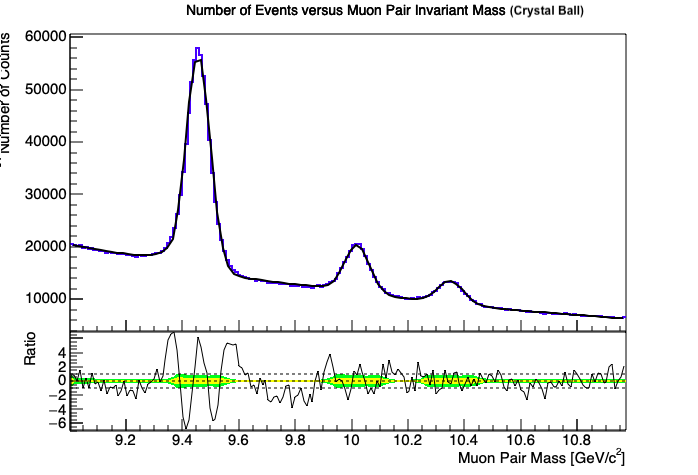
\includegraphics[width=0.7\columnwidth]{figures/xmass_hist_cb.png}
\caption{Histogram showing the crystal ball function curves fit to the three peaks, along with the exponential background fit.}
\label{fig:2d_hists_ex}
\end{figure}

 The values of \textalpha\ and $n$ are determined by fitting a Crystal Ball to the Monte-Carlo (MC) simulation data. These two parameters are then used to fit the actual data. The crystal ball fit resulted in a $\chi ^2$ value of 5.003.\\